\chapter{Lower Hybrid and Current Drive}


\section{Introduction}
Originally, the occurrence of a wave resonance, the \emph{lower hybrid resonance}, has been anticipated to lead to strong wave-particle interaction through linear and non-linear mode conversion to a hot plasma wave \parencite{Stix1992}. With an appropriate RF launcher conceived to excite cold plasma waves, these would propagate into the plasma until reaching the lower hybrid resonant layer at $\omega_{LH}$. This resonance exists in tokamak plasma in the region close to the ion plasma frequency $\omega \pi/2\pi$ , which lies in the lower end of the microwave band (1-5 GHz). At this layer, the perpendicular group velocity vanishes and the waves can convert into a hot plasma mode which is absorbed. This heating technique, known as \emph{Lower Hybrid plasma Ion Heating} (LHIH) or \emph{Lower Hybrid Resonance Heating} (LHRH), was the originally experimentally investigated method in the 70' \parencite{Bellan1974, Hooke1972, Golant1972, TONON1977, Schuss1981}. Different physical mechanisms have been invoked to explain the energy absorption, such as stochastic Ion Heating\parencite{Karney1977b,,Karney1978a, Karney1979c} and quasi-linear electron Landau damping \parencite{Brambilla1983, Fisch1978, Karney1979}.

In the 80', effective ion heating had only been obtained in a small number of experiments and research along the application of LH waves towards bulk ion heating were slowing down \parencite{Gormezano1986, Porkolab1984a, Tonon1984}. The reason for this is that bulk ion heating near the mode conversion layer appeared to be less reproducible and more difficult to achieve than electron heating. Indeed, as the wave frequency gets closer to the lower hybrid frequency, the shorter wavelength waves may be more effectively absorbed and/or scattered near the plasma surface by nonlinear effects such as parametric instabilities, low-frequency fluctuations, etc. Moreover, for LH bulk ion heating, the unconfined ions impinging on the wall induced a large amount of metallic impurities and then the increase of power radiated by the plasma.

Rather than trying to heat ions, it was theorized postulated that high phase velocity waves traveling in the direction parallel to the magnetic field could interact quasi-linearly by Landau interaction with the electrons population, and, by using an asymmetric spectrum could drive a large amount additional of toroidal plasma current \parencite{Fisch1978}. In the same fashion that for LHRH, the RF power is coupled to the plasma via launchers made of rectangular waveguides stacked periodically in the horizontal direction parallel to the toroïdal magnetic field. However, at the contrary of LHRH launchers, the LH waves are launched preferentially in one toroidal direction by mean of a phased array. The LH wave excited by such an array has an asymmetric parallel spectrum. The LH waves create an asymmetry in the electron distribution, which ultimately results in a net electric current \parencite{Fisch1987}. This technique is known as \emph{Lower Hybrid Current Drive}\footnote{Despite the fact that the Lower Hybrid resonance is not any more involved in the use of this method in tokamaks, the term remained.} (LHCD) and has been confirmed on the PLT tokamak in 1982 \parencite{Bernabei1982, Motley1985, Jobes1985} and in Alcator C in 1984 \parencite{Porkolab1984}. 

Since in 1982 many impressive results were presented on LHCD\parencite{Hooke1982, Porkolab1984, Tonon1982} toward steady state or quasi steady state tokamak operations, most LH experiments were dedicated to electron interaction and especially to current drive. A recent review of LHCD is available in \parencite{Bonoli2014}.

Currently, the Lower Hybrid waves term refers to the waves which satisfy the slow-wave branch of the cold plasma dispersion relation for parallel index larger than one ($|n_{\parallel}|>1$) and a RF frequency $\omega$ which lies between the ion cyclotron $\omega_{ci}$ and the electron cyclotron $\omega_{ce}$ frequencies. 

For the LH (lower hybrid) method which operates at the lower end of the microwave band (1-5 GHz) klystrons transform electrical power into electromagnetic power (step 1), which is transported to the plasma using waveguides (step 2). The power is coupled to the plasma with antennas called "grills" because of their characteristic shape (step 3), transported inside the plasma by plasma waves (typically the slow wave) (step 4), and absorbed on ions or electrons by wave-particle interaction (step 5).

\section{Klystrons}
A klystron is a vacuum tube used as amplifiers at narrow band microwave and radio frequencies. In the fusion domain, they are used mainly to produce high power waves, at the level of hundred of kilo watts during many seconds. First klystrons have been invented by the Varian brothers in 1937 \parencite{Pond2008}. The first klystrons have been intensively used during World War II, as RF power generators for RADAR systems. Klystrons sources between 2.45 GHz and 5 GHz are now available at the 0.5-0.8 MW/10-1000 s level\parencite{Pond2008}. 

The principle of a klystron is illustrated in Figure \ref{fig:klystroncut} \parencite{Tenenbaum2003} and detailed below:

\begin{enumerate}
 \item  A continuous electron beam is emitted by the klystron's cathode and accelerated to high voltage in a DC gun 
 \item The electron beam passes through a resonant cavity (input cavity) which is excited by an external source of RF power (typically in the milliwatt to the watt range) at the resonant frequency of the cavity (resonant cavity) 
\item While passing through the first cavity, the electron beam velocity is modulated by the weak RF signal: the sinusoidal variation in the cavity voltage causes alternate acceleration and deceleration of electrons in the beam. 
\item The beam passes through a drift tube, in which the accelerated electrons travel faster and the decelerated ones travel slower, resulting in a beam which is bunched at the frequency of the RF drive signal; thus a significant fraction of the beam’s power has been moved from DC to the drive frequency. 
\item The beam passes through a series of cavities in which are induced standing waves at the same frequency as the input signal. The signal induced in the second chamber is much stronger than that in the first, thus leading to amplification of the velocity and density modulation of the beam. A larger number of cavities may be used to increase the gain of the klystron, or to increase the bandwidth. 
\item The output cavity is located at a point where the electron bunches are fully formed. The resonant frequency of the output cavity is the same as that of the input cavity and the power is transferred from the beam to the output cavity. 
\item The RF power extracted from the output cavities travels to an output waveguide(s) and exits the klystron body.;  since the klystron us vacuum pumped, a RF window is necessary. RF feed-troughs (or “windows”) are mounted at the RF outputs to ensure the transition between the vacuum inside the tube and the pressurized waveguides.
\item The residual electron beam energy is dissipated in an actively cooled collector. spent beam is transported to a collector, which is a water-cooled beam stop. 
\end{enumerate}

\begin{figure}
\centering
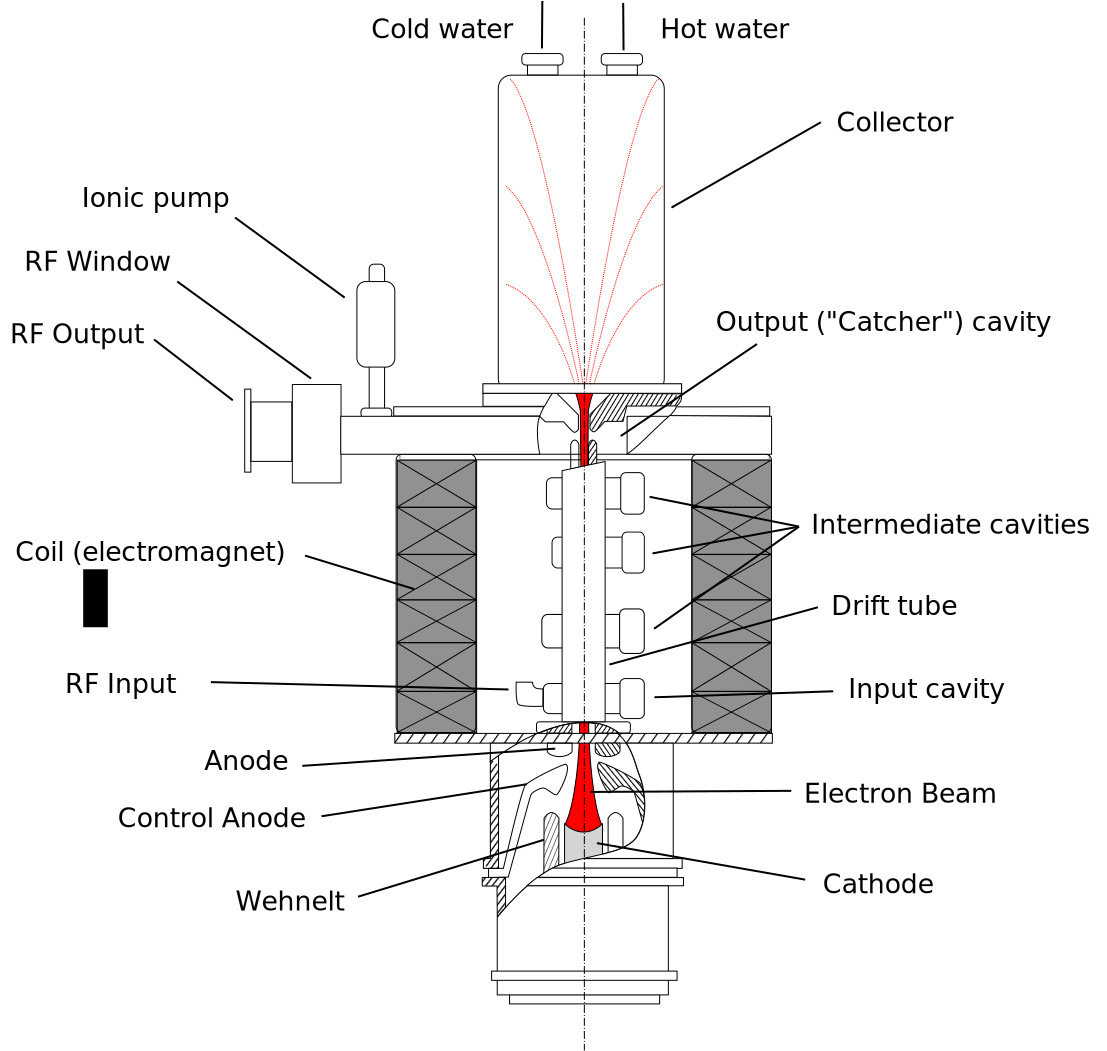
\includegraphics[width=0.6\linewidth]{Figures/LHCD/klystron_cut}
\caption{Schematic cut of a klystron.}
\label{fig:klystroncut}
\end{figure}


\begin{figure}
\centering
\includegraphics[width=0.7\linewidth]{Figures/LHCD/TH20103_TH20103C}
\caption{Two Klystrons used in the Tore Supra tokamak LH system. Left: 500kW/210s klystron (1980'); right: 700kW/CW klystron (2002). Both have been manufactured by Thales Electron Device. 16 of each model have been installed in the Tore Supra LH plant. These klytrons require a high voltage supply of 60 to 76kV (cathode voltage) for 2220-22 A (beam current). Their gain is greater than 50 dB for an efficiency of 40-45\%.}
\label{fig:th20103th20103c}
\end{figure}


\section{LH Transmission Lines}
As the RF frequency increases, coaxial cable losses (expressed in decibel per distance in Figure \ref{fig:rfcafetlattenuations}) become unpracticable for high power applications. In the LH range of frequencies (1-5 GHz), hollow rectangular waveguides are preferred for the transport of the RF power from the klystrons to the torus. In addition to their low losses, they also allow a greater breakdown voltage than coaxial lines of the same size. In this frequency range the wavelength in vacuum is of the order of 30 cm to 6 cm.


\begin{figure}
\centering
\includegraphics[width=0.9\linewidth]{Figures/LHCD/RFCafe_TL_attenuations}
\caption{Various transmission line attenuation vs frequency. Source: \url{http://www.rfcafe.com/references/electrical/ew-radar-handbook/microwave-waveguide-coaxial-cable.htm}.}
\label{fig:rfcafetlattenuations}
\end{figure}


\subsection{Rectangular waveguides} 
A hollow rectangular waveguide of width a and height b is illustrated in Figure \ref{fig:rectangularwaveguide}. Solving Maxwell’s equations for this geometry leads to multiple possible solutions, or \emph{modes}. These modes are eigenfunctions of the equation system. Each mode is characterized by a cut-off frequency, below which the mode cannot propagate in the guide. In a rectangular waveguide, modes can be expressed as \emph{Transverse Electric} (TE) or \emph{Transverse Magnetic} (TM), depending of their respective polarization. Since the walls of a rectangular waveguide constrain the electromagnetic field boundary conditions along two dimensions, two integer indices are used to describe a mode from another. Thus, modes in a rectangular waveguides can be $\mathrm{TE}_{10}$, $\mathrm{TE}_{20}$, $\mathrm{TM}_{11}$, etc. 

For practical applications, the dimensions of the waveguides are generally chosen in order to have one and only one mode allowed propagating for a specified frequency band. This single mode is the first one to appear to be propagating, and is referred as the \textit{fundamental mode} (generally labelled TE10). Other modes can eventually be excited by waveguides discontinuities, but can’t propagate since they are evanescent. They are referred to \textit{high order modes}.

For high power applications, a great care is given to waveguide inner walls, bends and connections, since reflected power and arcs may occur due to discontinuities in the conducting walls, such as the ones caused by misalignments, bumps, holes, etc.

\begin{figure}
\centering
\includegraphics[width=0.5\linewidth]{Figures/LHCD/Rectangular_Waveguide}
\caption{Illustration of a rectangular hollow waveguide. Source:Wikipedia.}
\label{fig:rectangularwaveguide}
\end{figure}


\subsection{Waveguide plumbery – a practical example with Tore Supra}
Many waveguide devices have been developed in order to transmit, measure, combine or split the power from one point to another. These devices are commonly used on LHCD systems to transport the power from a klystron to (a section of) an antenna, but also in order to protect the klystron from possible reflected RF power by the plasma.   

As an example of the usage of such devices, the Tore Supra LHCD system is illustrated in Figure \ref{fig:toresupralhcdsystem}. The power is generated at the klystron plant and transmitted to the two launchers through rectangular waveguides (8 lines per launcher). 

\begin{figure}
\centering
\includegraphics[width=0.9\linewidth]{Figures/LHCD/ToreSupra_LHCD_System}
\caption{Schematic of the Tore Supra LHCD system, from the klystrons plant to the vacuum vessel.}
\label{fig:toresupralhcdsystem}
\end{figure}


Once reaching the launcher rear end, the power goes trough a \textit{hybrid junction} (also called 3-dB splitter). This device splits the incident power into two waveguides, one to feed the upper part and the other for the lower part of the launcher.  If reflected power (from the plasma) returns from these two waveguides, the power is recombined and directed to a fourth one. An actively cooled water load is connected to this fourth port, in order to dump the remaining RF power reflected by the plasma and thus protect the klystron. A rectangular waveguide 3-dB splitter is illustrated in Figure \ref{fig:hybridjunction1}. 

\begin{figure}
\centering
\includegraphics[width=0.4\linewidth]{Figures/LHCD/HybridJunction1}
\includegraphics[width=0.4\linewidth]{Figures/LHCD/HybridJunction2}
\includegraphics[width=0.4\linewidth]{Figures/LHCD/HybridJunction_Efield}
\caption{Top: Illustration of an rectangular waveguide hybrid junction. When excited from port 1, the power is split to ports 2 and 3. when the power comes from ports 2 and 3, the power is recombined and directed to port 4, where the power is dumped into a water load. Bottom: The electric field distribution when excited from port 1. }
\label{fig:hybridjunction1}
\end{figure}


After being split, the RF power goes through various devices up to the plasma (Figure \ref{fig:toresuprac4cad}): 
\begin{itemize}
\item A bidirectional coupler, which allows measuring the forward and reflected power amplitude and phase ;
\item A DC break, which isolates the DC potential of the tokamak from the DC potential of the transmission line (for the protection of persons);
\item A vacuum feed through (window) which isolates the tokamak vacuum from the pressurized medium existing in the waveguide. These windows (16 by launchers) are illustrated in Figure \ref{fig:toresuprac4cad}. A window consists in a dielectric medium inserted between two rectangular waveguides. The dimensions of the dielectric medium (a ceramic, such beryllium oxide BeO or alumina) are calculated in order not producing reflected power. A part of the power is always absorbed in the ceramic, so a great care is applied to correctly cool the window in order to avoid heating up and ultimately break the ceramic.
\item A TE10-TE30 mode converter, which splits the incoming RF power into three, thus leading to split the power into three poloidal rows of waveguides. A mode converter is a rectangular waveguide device which large side is modulated in order to allow higher modes (such as TE20, TE30 and TE40) and such that the power is totally transferred from one mode to another one (efficiency is close to 100\%). Once the power is transferred to the TE30 mode, metallic septa located in zero field regions split the power into three independent waveguides. The device is illustrated in Figure \ref{fig:modeconverter}.
\item Finally a multijunction, a structure which will be described in details in the next section, splits and phases the power in the toroidal direction, then leads to the plasma. 
\end{itemize}


\begin{figure}
\centering
\includegraphics[width=0.9\linewidth]{Figures/LHCD/ToreSupra_C4_CAD}
\caption{Illustration of the power splitting scheme in Tore Supra LHCD launcher C3 or C4.}
\label{fig:toresuprac4cad}
\end{figure}


\begin{figure}
\centering
\includegraphics[width=0.9\linewidth]{Figures/LHCD/ModeConverter}
\caption{Illustration of the electric field distribution in a TE10-TE30 mode converter at 5 GHz. The device is excited from the left.}
\label{fig:modeconverter}
\end{figure}


\section{LHCD launchers}
\subsection{“Grill” launchers}
As the plasma cross-section dimensions of toroidal devices became sufficiently large to accommodate the free space wavelength at the lower hybrid frequencies, it becomes possible to couple the RF power directly by open-ended waveguides inserted in the vacuum vessel wall, thus avoiding coils or antennas within the vacuum chamber\footnote{To give some numerical orders, the COMPASS-D tokamak, operated in Culham from to 1989 to 2001, used 1.3 GHz RF power sources, and rectangular waveguides of cross-section 165x82mm to carry the RF power to the LH launcher. Smaller wavelengths (i.e. higher frequency sources, up to 8 GHz) have been used, leading to smaller waveguides cross-section.}.
 
However, in order for the wave to access from outside the plasma to inside the plasma, the wave has to be “slowed down” along the static toroidal magnetic field. This means that the parallel phase velocity of the wave $v_{\parallel}$ has to be reduced with respect to the speed of light $c_0$, in order to being able to penetrate trough the plasma. It is said that the waves must satisfy an \emph{accessibility condition} \parencite{Golant1972, Stix1992}\footnote{The accessibility condition is sometime referred as the Golant's accessibility criterion, for e.g. in\parencite{Puri1974}.} Equivalently, this condition requires for the wave to have a sufficiently large refractive \emph{parallel index} $n_{\parallel} = c_0/v_{\parallel} = k_{\parallel}/k_0$, parallel to the magnetic field. The use of a phased array as a way to slow down the waves and thus to launch LH waves was first suggested by Lallia\parencite{Lallia1975} and investigated by Bernabei et al. in 1975\parencite{Bernabei1975}. Lallia suggested that a set of properly phased waveguides, called "grill"\footnote{The similarity to the cooking utensil leads to nickname these launchers "grill".}, would efficiently slow down the wave parallel to toroidal magnetic field. The short sides of the waveguides are mounted parallel to the toroidal magnetic field, to launch effectively a slow wave mode into the plasma. 

The coupling is the process by which RF power propagates and possibly tunnels from an antenna to the plasma \parencite{Meneghini2012}. Brambilla developed the theory of the coupling of  a simplified grill structure to a large toroidal plasma \parencite{Brambilla1979} \footnote{The Brambilla theory has been applied (and still) to many different geometries, from single waveguide to hundred of waveguides array. Some examples are cited here, like a 2-waveguides array with one mode in \parencite{Krapchev1978} or to 16-waveguides array in \parencite{Stevens1988}.} This coupling theory has been generalized later to the fast wave coupling \parencite{Theilhaber1979,Theilhaber1980} and to 3D rectangular waveguides in \parencite{Bers1981, Bers1983}. 

Several important remarks can be drawn from the properties of the propagation of cold-plasma waves into the plasma. The wave is evanescent if the electron density is below a cut-off density $n_{\mathrm{cutoff}}$. However, if such a low density layer is thin enough, the wave can tunnel through it. Thus, similarly to ICRF antennas, the LH launcher must be close enough of the plasma\footnote{Or the plasma local density must be increased by gas puffing.} in order to efficiently couple high power. 

In these conditions, the thermal and mechanical stresses are essential parameters to design an LH launcher. They and constitute a challenge to deliver such for these systems in for fusion reactors. As for ICRH antennas, LHCD launchers distributed in the vacuum vessel is being proposed for DEMO, mitigating substantially these issues.

Different types of grills have been developed to accommodate the conditions that the wave must be coupled to and (then) propagate in the plasma. 

\begin{figure}
\centering
\includegraphics[width=0.4\linewidth]{Figures/LHCD/COMPASS_grill_out}
\caption{Picture of the grill mouth of the COMPASS-D LH launcher, made of 8 waveguides. Generator frequency was 1.3 GHz.}
\label{fig:compassgrillout}
\end{figure}

\begin{figure}
\centering
\includegraphics[width=0.7\linewidth]{Figures/LHCD/CMod_LH1}
\caption{The Alcator C-Mod LH1 launcher (88 waveguides, 4.6 GHz) and it associated transmission line (aka the”jungle gym”).}
\label{fig:cmodlh1}
\end{figure}

\subsection{Multijunction Launchers}
In a large tokamak, a conventional LH grill made of independently fed waveguides would require hundred of waveguides, leading to a very complex power splitting design behind the antenna (cf.Figure \ref{fig:cmodlh1}). The use of \emph{multijunction} grill was suggested in 1984 to overcome this limitation \parencite{Gormezano1985, Moreau1984}. In a multijunction grill, the main waveguide is divided into $N$ smaller (secondary waveguides) by thin metallic walls parallels to the wall of the main waveguide and perpendicular to the electric field: the \emph{E-plane N-junctions}. Built-in phase shifters made by reducing the waveguide height (in order to increase the guided wave phase velocity) are added in the structure in order to obtain the desired output phasing of the grill. Multijunction launcher makes it simpler to create and feed a large number or waveguides, at the contrary of classic grills launchers. However, a drawback is that the adjustment range of the power density spectrum is limited to a smaller range than for classic grills launchers.

A judicious choice of the phasing of the output waveguides leads to an important self-matching property of the multijunction (also known as \emph{recycling effect} or \emph{load resilience}). Indeed, for specific phase values, the reflected waves from the plasma which return back in the secondary waveguides can be reflected back to the plasma, thus leading to multiple reflections in the secondary waveguides. This recycling effect, which takes place between the plasma-antenna discontinuity and the E-plane bi-junctions, leads to an attenuation of the waves at each passage by the plasma, and ultimately to a decrease of the reflected power toward the RF sources. 

TODO: Illustration of the recycling effect (load resilience) inside a multijunction.


\begin{figure}
\centering
\includegraphics[width=0.3\linewidth]{Figures/LHCD/ToreSupra_C2}
\includegraphics[width=0.4\linewidth]{Figures/LHCD/ToreSupra_C3}
\caption{Left:The Tore Supra Multijunction launchers as view from inside the vacuum vessel. The C2 launcher (128 waveguides, total dimensions 50 x 40 cm, 1989). Right: The C3 launcher (288 waveguides, total dimensions 60cm x 60cm, 1999). Frequency: 3.7GHz.}
\label{fig:toresupraC2C3}
\end{figure}


\subsection{Passive-Active waveguide array launchers}
One of the main show-stopper to the use of LHCD to realize long and efficient pulses (outside the constraints of the tokamak magnetic coils heating) is the ability to couple high LH power to the plasma. Indeed, in order to achieve good coupling, the electron density in front of the LH launchers needs to be large enough, which means that the launcher needs to be located close enough to the plasma or to increase the local density by gas puffing means. 

The alternation of \emph{passive} waveguide (a waveguide closed by a short-circuit) and \emph{active} waveguide (a waveguide that is directly fed from the generator) has been initially proposed by Motley and Hooke \parencite{Motley1980} in order to minimize the \emph{surface wave} excitation. Moreover, it was found that adding passive waveguide at each side of the array leads to decrease the reflected power in the last active guide \parencite{Krapchev1978, Motley1980B}. The passive waveguides act as reflectors, radiating back a part of the power reflected by the plasma, and thus improving the coupling efficiency. Passive-Active grills were envisaged since the 1980' for fusion-reactor grade devices \parencite{Ehst1982}. In these first conceptual designs, the passive waveguides were thought to be plugged or tuned individually in order for the outgoing power to have the requisite phase corresponding to an all-active grill system. 

Being close to the plasma leads to increase the heat fluxes into on the launcher front face. Thus, in order to improve the cooling of the launcher front face, it has been proposed in 1995 to insert one passive waveguide between each active waveguide, behind which a water pipe could efficiently water-cool the structure \parencite{Bibet1995}. 

In order to insure a lower reflected power than a conventional grill, it has been proposed to associate this alternation of passive-active waveguide to  use a multijunction. This Passive-Active Multijunction (PAM) concept addresses two of the main criticisms made to LH launchers, i.e. the coupling efficiency and the heat loads resilience. 



\begin{figure}
\centering
\includegraphics[width=0.4\linewidth]{Figures/LHCD/Pam_FTU}
\caption{PAM prototype tested on the FTU tokamak (24 active waveguides, 24 passive waveguides, 8 GHz, 2003) \parencite{Mirizzi2003, Ridolfini2005}.}
\label{fig:pamftu}
\end{figure}



\begin{figure}
\centering
\includegraphics[width=0.6\linewidth]{Figures/LHCD/dsc_6078_dxo_2}
\includegraphics[width=0.3\linewidth]{Figures/LHCD/ToreSupra_C4}
\caption{The Tore Supra PAM (C4) launcher (96 active waveguides, 102 passive waveguides, approx. 7 tons, front face dimensions 60cm x 60cm, 3.7 GHz, 2009) \parencite{Guilhem2009, Guilhem2011}.}
\label{fig:toresupraC4}
\end{figure}


\subsection{Poloidal splitter launchers}
Motivated by the reduction of the RF losses and the increase of the reliability of a LH launcher, while keeping the flexibility in the parallel index $n_{\parallel}$ spectrum of the “grill” configuration (at the contrary of multijunction), the Alcator C-Mod team developed in 2008 a launcher (LH2) based on a four way splitter \parencite{Koert2008a}. At the contrary of multijunction launcher, the four way splitter divides the power in the poloidal direction. Since the power splitting is done poloidally, the launched parallel power spectrum can be changed with the same flexibility as with conventional grill antennas. This design simplified the feeding structure of the antenna, thus reducing the RF losses due to multiple power splitters and flanges of previous grill configurations, while keeping a simple manufacturing assembly. The RF power is redistributed depending on the plasma load on each of the four rows of the splitter. If the load is the same for each row, the power is evenly split among rows. The RF optimization of the launcher has been made for a source frequency of 4.6 GHz and assuming a simplified plasma load (constant) in front of each row. A similar design has been made for the KSTAR tokamak, at 5 GHz \parencite{Kim2012}. 


\begin{figure}
\centering
\includegraphics[width=0.4\linewidth]{Figures/LHCD/FourWaySplitter_1module}
\includegraphics[width=0.4\linewidth]{Figures/LHCD/FourWaySplitter_CAD}
\caption{Left: CAD conceptual schematics of the four-way splitter of Alcator C-Mod \parencite{Koert2008a}.Right: final assembly CAD model with 16 four-way splitters \parencite{Meneghini2010b}.}
\label{fig:fourwaysplitter1module}
\end{figure}


\begin{figure}
\centering
\includegraphics[width=0.4\linewidth]{Figures/LHCD/CMod_LH2}
\caption{Picture of the LH2 launcher inside the Alcator C-Mod vacuum vessel with its lateral protections in January 2012 \parencite{Meneghini2010b}.}
\label{fig:cmodlh2}
\end{figure}


\section{Wave propagation and absorption in the plasma}
In order for the RF power to reach the plasma core, the excited waves by a LHCD launcher must satisfy different criteria: 

\begin{itemize}
\item  A \emph{cut-off condition}: the electron density in front of the launcher must be close or higher than the slow-wave electron \emph{cut-off density}. This density is given by:
$$
n_{c,\mathrm{cut-off}} = \varepsilon_0 m_e \frac{\omega^2}{e^2}
$$
and thus increases as the square of the source frequency. 
\item A propagation condition: in order for the LH waves to propagate into the magnetized plasma, excited waves must have an absolute value of the parallel index greater than one, i.e. $|n_{\parallel}|>1$ 
\item An accessibility condition: in order for the slow waves which access to the core plasma not to be mode-converted into fast waves, a minimum value of $n_{\parallel}$ for a given plasma density and magnetic field is requested :
$$
|n_{\parallel} |>| n_{\parallel \mathrm{access}} | 
\approx 
\sqrt{1 
	- \frac{\omega_{pi}^2}{\omega^2} 
	+ \frac{\omega_{pe}^2}{\omega_{ce}^2}}
+ \frac{\omega_{pe} }{| \omega_{ce} |}
$$ 
When the accessibility condition is satisfied, the slow and the fast branch of the dispersion relation are separated and the LH waves can reach the core plasma.
Inversely, for a given $n_{\parallel}$, the previous condition leads to an upper limit for the density, above which the wave can’t propagate.
\end{itemize}

\begin{figure}
\centering
\includegraphics[width=0.9\linewidth]{Figures/LHCD/C3_powerflow}
\caption{Illustration of the power density radiated by a LH launcher (seen into a horizontal plane cut) into a plasma of increasing electron density. The plasma current direction is indicated. Since the launcher is designed to launch a non-symmetrical power spectrum, the power flows toward a preferred direction (opposite to the plasma current).}
\label{fig:c3powerflow}
\end{figure}



The RF power is coupled by the launcher to the plasma, which means that the electromagnetic waves in the launcher’s waveguides are converted to (mainly) slow waves in the plasma. In the LH range of frequencies (~2 to 8 GHz), the wavelength of the RF waves in the plasma is well below the typical beam size, which itself is smaller than the equilibrium non-uniformity scale. It this situation, the evolution of the waves in the plasma can be described by the \emph{ray-tracing} formalism. Since the evolution of the electron population can be described with Fokker-Planck calculation, the combination of the both tools is standard for modelling LHCD experiments\parencite{Bonoli1982, Peysson2012}.

As said before, the LHCD launcher is a phased array of waveguide which excites a slow plasma wave. The following calculations taken from current drive theory illustrate the basic requirements of the LHCD launcher in order to optimize the current drive efficiency. 

In the plasma, the incremental current $\Delta j$ carried by an electron of electrical charge $q=-e$ and accelerated from a parallel velocity $v_\parallel$ to $v_\parallel + \Delta v_\parallel$ is:
$$\Delta j = q \Delta v_{\parallel}$$

The incremental increase of kinetic energy is:
$$\Delta E = m v_{\parallel} \Delta v_{\parallel}$$

Eliminating $\Delta v_{\parallel}$ leads to an incremental current: 
$$\Delta j = \Delta E \; q/(m v_{\parallel})$$ 

Let $\nu_\mathrm{coll}$ be the Coulomb collisional frequency. At first order \footnote{Rigourously, the mathematical tool for a complete description of multiple scattering processes in the velocity-space is the Boltzman equation. The collision term modelling the multiple particles Coulomb collisions in this equation can be modelled by a collision term of the Fokker-Planck type.} the incremental energy input $\Delta E$ persists for a time $1/\nu_\mathrm{coll}$. The associated (steady-state) RF input power $\Delta P$ required is thus: 
$$\Delta P = \nu_\mathrm{coll} \Delta E$$ 

From the two previous equations, the ratio of the incremental current to the RF input power is:
$$\Delta j/ \Delta P = q / (m \nu_\mathrm{coll} v_{\parallel})$$

This suggests that more current can be driven with low parallel velocity electrons. However, fast electrons collide less often than slower, as the Coulomb collision cross section falls off with increasing relative velocity as $\nu_\mathrm{coll} \propto n_e/v_{\parallel}^3$ (for parallel velocity larger than the thermal velocity). It follows that the previous ratio is proportional to: 

$$\Delta j/ \Delta P \propto (v_{\parallel}^2 q) / (m n_e)$$

this means that high current drive efficiency can be reached from fast electrons. Thus, it is actually more effective to push fast electrons than slower. Even if it may be energetically more expensive to accelerate fast electrons, this energy deposition need occurs less often because current last longer when carried by relatively less collisional electrons \parencite{Fisch1987}. 

For the purpose of current drive with LH waves, the Landau damping is the dominant absorption mechanism. Landau damping is a collision-less damping process in which particles exchange energy with waves travelling with the nearly same phase velocity parallel to the magnetic field, that is, for particle parallel velocity $v_{\parallel}$ satisfying resonant condition:

$$\omega – k_{\parallel} v_{\parallel} = 0 $$ 

where $k_{\parallel}=k_0 n_{\parallel}$ is the parallel wavenumber of the wave, $n_{\parallel}$ the parallel index of refraction and $k_0= \omega/c$ the wavenumber in vacuum. From the previous relation one deduces that the LHCD launcher must excite waves satisfying the resonant condition $v_{\parallel}=c/n_{\parallel}$. As for the slow wave to be able to penetrate into the plasma the parallel index must be greater than one and also greater to $|n_{\parallel \mathrm{access}}|$, typical LHCD launchers in current tokamaks excite a main parallel index between $n_{\parallel 0}$=1.5 to 3.0. 

However, in many past and present LHCD experiments, the resonant velocity $v_{\parallel 0}=c/n_{\parallel 0}$ corresponds to supra thermal region where the number of electrons should be in principle too small for any significant wave damping to take place and to account for the observed current drive. Indeed, strong wave damping on a Maxwellian distribution with temperature $T$ requires the wave damping to be no larger than four times the thermal velocity $v_T=\sqrt{k T/m}$. This paradox is commonly referred to as the \emph{spectral gap} problem and is an active area of research. Various explanations are proposed to explain this spectral gap, among these the toroidal effects on the wave propagation that can cause sufficient up-shift (increase of the parallel wavenumber) in the parallel refraction index $n_{\parallel}$ to “fill” the spectral gap, non-linear interactions such as \textit{parametric decay instabilities} (PDI), diffraction effects or power density spectrum fluctuations. 


\section{Overview of parameters achieved and example of some systems}
\subsection{LH Launchers main figures of merit}

There are three important figures of merit to measure the efficiency and the performances of a LH launcher: 
\begin{enumerate}
	\item The first one is the k-space radiated power spectrum, generally characterized by its \emph{parallel power spectrum} $p(n_{\parallel})$ . This quantity represents the amount of power for each parallel index excited by the launcher. The relation between this power spectrum and the array excitation is related to the Fourier transform of the electromagnetic field at the plasma-antenna interface. 

	\item  The second one is the ratio of the reflected power (at the mouth or at the end of the launcher) to the input power, named the \emph{reflection coefficient} (sometime expressed in percent). 
$$RC = \frac{P_r}{P_i}$$
	\item The third one is the \emph{directivity} of the launcher, which is the fraction of the power spectrum over its total power content. It can be viewed as the fraction of the power that goes toward one toroidal direction over the total coupled power. One can define the directivity as follow\footnote{Other definitions exist, essentially in order to ad a physical content to the directivity, in relation with the current drive efficiency evolution in the plasma. See for instance \parencite{Litaudon1990a}.}
$$
D
= 
\frac{
	\int_{n_{\parallel} >0} p(n_{\parallel}) dn_{\parallel} 
	}{
	\int_{n_{\parallel}} p(n_{\parallel}) dn_{\parallel} } 
$$
\end{enumerate}

Theoretically, if the $n_{\parallel}$ spectrum of an antenna is known, one can evaluate the reflection coefficient. However, since the wave field at the launcher aperture (and thus the launcher spectrum) depends on the plasma itself, numerical codes are required to make a self-consistent numerical evaluation of the coupling. Such codes are coupling codes.

\subsection{LH systems and launchers performances}
Mainly because of its relative simplicity, most of the LH launchers have been based on a “grill” configuration, as for example in the 1980' \parencite{Porkolab1984a, Gormezano1986a, Stevens1988}\footnote{It is a non exhaustive list.}

Typical grill launchers have a high reflection coefficient (of the order of 20 to 40\%) but directivity higher than 80\%. Since all the waveguides can be feed by independent RF sources, and thus independently phased, such launchers have a wide flexibility in terms of operational space (excited spectrum) which is of great interest for physics studies. However, since each waveguide is independently power fed, the complexity of the launcher grows enormously with the number of output waveguides, leading to cumbersome transmission systems for multi-megawatt power levels (Table \ref{tab:grillperformances}). 

\begin{table}
	{\rowcolors{2}{LightYellow1}{LightYellow2}
		\begin{tabular}{| p{6cm} | p{5cm} |}
			\hline 
			Launcher & Total number of waveguides \\
			\hline \hline
PLT Grill 1 (1981-1984)  \parencite{Stevens1988} & 6 (0.8 GHz) \\
			\hline
PLT Grill 4 (1986) \parencite{Stevens1988} & 16 (2.45 GHz) \\
			\hline
COMPASS-D (1989) & 8 (1.3 GHz) \\
			\hline
Alcator C \parencite{Porkolab1984a} & 16 (4.6 GHz) \\
			\hline
Alcator C-Mod LH1 (2006) & 88 (4.6 GHz) \\
			\hline
		\end{tabular}
	}
\caption{Waveguide number and maximum performances in some grill launchers.}
\label{tab:grillperformances}
\end{table}

Multijunction launchers at the contrary have led to hundred of waveguides launchers (see Table \ref{tab:multijunctionperformances}). The complexity of the multijunction design and manufacturing is balanced by the a simpler transmission line system behind the launcher. Because of the self-matching property, the typical reflection coefficient of multijunction launchers is generally less than 10\%. However, the multiple back and forth of the waves leads to an increase of the peak electric field in secondary waveguides. Moreover, since the phase shift is created by the built-in phase shifter inside the launcher, the flexibility of phase configuration is reduced in comparison to classic grill launchers. 

\begin{table}
{\rowcolors{2}{LightYellow1}{LightYellow2}
\begin{tabular}{| p{6cm} | p{5cm} |}
	\hline 
Launcher	& Total number of waveguides  \\ 
	\hline \hline
Petula-B \parencite{Gormezano1985}	& 4 (1.3 GHz)    \\ 
	\hline 
JT60 CD-3 \parencite{Ikeda1989}	& 24x4=96 (1.74-2.23 GHz)    \\ 
	\hline 
JET \parencite{Litaudon1990a}	& 2x2x2x6x8=384 (3.7 GHz)   \\ 
	\hline 
Tore Supra C1 and C2 \parencite{Litaudon1992a}	& 4x2x8x2=128 (3.7 GHz)   \\ 
	\hline 
Tore Supra C3 \parencite{Bibet2000}	& 6x3x8x2=288 (3.7 GHz)   \\ 
	\hline 
EAST & 8x4x5=160 (2.45 GHz) \\
	 & (4.6 GHz) \\
\hline
\end{tabular} 
}
\caption{Waveguide number and maximum performances in some multijunction launchers}
\label{tab:multijunctionperformances}
\end{table}

\begin{table}
		\begin{tabularx}{\textwidth}{|X|X|X|X|X|X|}
			\hline
Tokamak	& Number of sources & Total installed power (MW) &	Frequency range (MHz) &	Number and type of antenna & 	Max. pulse Length (s) \\
			\hline\hline
JET				& 24	& 15	& 3.7 	& 1 MJ	& 13  	\\
Tore-Supra 		& 16 	& 9		& 3.7	& 1 MJ 	& 		\\
				&    	&  		&      	& 1 PAM 			& 390 	\\
Alcator C-Mod	& 8		& 2		& 4.6	& 1 grill			& 		\\
EAST			& 20 	& 4 	& 2.45 	& 1 grill 			& 		\\
				& 24	& 6 	& 4.6	& 1 MJ	& 400 	\\
HL-2A 			& 4 	& 1.6	& 3.7	& 1 PAM 			& 		\\
SST-1 			& 4 	& 2		& 3.7 	& 1 grill			&	 	\\
KSTAR 			& 1 	& 0.5	& 5 	& 1 grill			& 		\\
ITER 			& 48	& 24 	& 3.7-5 & 1 PAM				& 1000 	\\
			\hline
\end{tabularx}
\caption{LHCD systems of JET, Tore Supra/WEST, Alcator C-Mod, EAST, HL-2A, SST-1, KSTAR and ITER}
\label{tab:recentLHCDsystems}
\end{table}

The PAM concept tested in FTU and in the Tore Supra tokamak showed that reflected power lower than 5\% (i.e. high coupling efficiency) and continuous operations could be combined (cf. Figure \ref{fig:ts45472c4ir}) during long pulse operations. 
\begin{figure}
\centering
\includegraphics[width=0.9\linewidth]{Figures/LHCD/TS45472_C4_IR}
\caption{Illustration of a Tore Supra discharge with the PAM launcher (TS\#45472, 2010) \parencite{Ekedahl2010b}. The design goal power density (25MW/m$^2$ ) is achieved during 78s, with very low reflected power (<2\% of the input power), even at large plasma launcher distance (~10 cm) (density is not the line-average density). The Infra-Red monitoring shows that the global temperature of the launcher mouth is lower than 270$^{\circ}$C, validating its efficient cooling structure.}
\label{fig:ts45472c4ir}
\end{figure}


\section{ITER System}

Although not part of the initial ITER planned procurement phase, a 20 MW/CW 5 GHz LHCD system is due to be commissioned and used for the second mission of ITER, i.e. Q=5 steady state target \parencite{Hoang2009}. In ITER, the parallel index of the launched waves $n_{\parallel 0}$ ~ 2.0 has been selected as a trade-off between the current drive efficiency, the wave accessibility and the location of power deposition, all of which depend upon the plasma conditions. Depending of the plasma scenarios (steady-state, hybrid, ramp-up, etc.), the additional current driven by LHCD would range between 0.42 MA (steady-state) up to more than 3.0 MA (ramp-up) \parencite{Decker2011}. In any case, these values confirm that for steady state scenarios, a substantial bootstrap current is required \parencite{ITERPhysics_Chap6}. The average current drive efficiency, which is the figure of merit of the LHCD, has been calculated to be $\eta \equiv 0.2 \times 10^{20} A m^{-2} W^{-1}$, similar to the ones measured in present days tokamaks \parencite{ITERPhysics_Chap6}. This value can be compared to other additional current drive scheme, such as NBI or ECCD. 

In addition, LHCD-assisted start-up could reduce the flux consumption during current ramp-up, resulting in a longer flat top or burn time. An early application of 20 MW LHCD during the plasma current ramp-up phase of the ITER reference scenario 2 is effective to reduce the flux consumption. An expected saved flux of 43Wb is equivalent to about 500 s of additional burn duration \parencite{Hoang2009}.

\section{Overall discussion on strength and weaknesses}
Nowadays, the main usage of Lower Hybrid waves concerns current drive applications, in relation to quasi or fully steady-state plasma physics and scenario development. For this reason, LHCD systems are common on superconducting tokamaks for steady-state experiments, from continuous wave RF sources to actively cooled transmission lines and launchers.  

In term of performances achieved, fully non inductive discharges of up to 3.6 MA in JT-60U and 3 MA in JET have been achieved with LHCD. Plasma currents of 0.8 MA and 0.27 MA have been sustained for more than 6 minutes in Tore Supra and EAST. At very low density, the tokamak TRIAM-1M sustains even a 5 hours discharge. The EAST team also demonstrated 30s long pulse H-mode operation and ELMs mitigation possibility using LHCD. The current drive efficiency of LH waves has been measured to be equal or greater of than for other systems.

The coupling of LH waves to the plasma is achieved by launchers, a phased array of rectangular waveguides. The coupling of LH launcher is well understood and code predictions are in good agreement with experiments. As mentioned above, the slow waves excited by the launcher can propagate only if the electron density facing the launcher is greater than a cut-off density, $n_{e, \mathrm{cut-off}} = 3.1\time10^{17} m^{-3}$ at 5 GHz for ITER. Launchers are affected by a rapid decrease of the coupling efficiency for lower density, since in this case the wave is evanescent. Multijunction launcher and latter PAM structures solved part of this problem, demonstrating a total reflected power less than few percent in a wide range of edge density. Moreover, additional gas injection in the vicinity of the launcher has also been demonstrated with success. In any case, the launcher still has to be close ($\approx$cm) of the plasma edge and thus has to handle large plasma heat fluxes. These heat fluxes can be sustained with actively cooled structure, such as demonstrated in a PAM. 

In a fusion reactor, additional neutron heating fluxes, possible interactions with alpha particles and material requirements (such as avoiding copper) are additional challenges. Distributed launcher designs in the vacuum vessel have been proposed to reduce the power density requirement imposed by the use of fixed-dimensions ports, thus reducing the risk of arcing. From the launcher technological point view, CW operations have been demonstrated but additional margins, required for an efficient use into a reactor, must be gained in terms of reliability. 



